\chapter{Introduction} 
\label{ch:introduction}

% Because of a bug --- Restore original headers:
\fancyhead[ER]{\sffamily\footnotesize{\leftmark}}
\fancyhead[OL]{\sffamily\footnotesize{\rightmark}}

Neoway Business Solution is a big data analytics company with a variety of products on several verticals such as Sales and Marketing, Risk and Compliance, Health and others. One of the products of the Sales and Marketing vertical is called On Target(OT), which recommends leads for the users, based on their portfolio of clients. The OT will search for leads in a subset of the whole Brazilian's market space, which is composed by all active companies. The user can narrow down the search space based on a set of filters. The Figure \ref{fig:braz-comps-venn-diagram} shows a Venn diagram that illustrate the subsets of the OnTarget. The \underline{Portfolio} set is composed by the user's clients; The \underline{Market} is where the OnTarget will search for the leads, it can vary from a set defined by the filters to all the Brazilian active companies (except the user's clients).

\begin{figure}[h]
   \centering
   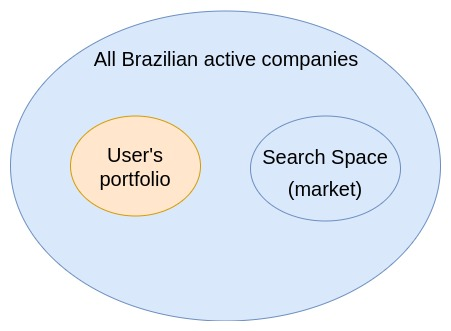
\includegraphics[width=9cm]{fig/ch1-brazil-comps-venn-diagram.jpg}
   \caption{Venn Diagram explaining the sets involved in the On Target product. Source: Author.}
   \label{fig:braz-comps-venn-diagram}
\end{figure}

Recently, OT was updated, and a benchmark was created to compare between different versions. Overall the new version showed an improvement in the performance of lead generation. However, at the same time, the new version yielded unexpected behavior, which suggests that the portfolio may present underlying clusters. The last point can be understood through Figure \ref{fig:simi-dist-expected-real} which shows two similarity distributions plots from the benchmark. Similarity is how similar a company on the market is with the user's clients, it ranges from 0 to 1. The blue curve shows the market distribution and the orange one the portfolio's sample distribution.\footnote{More about the similarity distribution plot will be explained on the chapter \ref{ch:methodology}.}
% OBS: "high density probabilities areas" = "bump"
(I) is the best case scenario of a study, where all the portfolio's samples are close to similarity 1; The market has two high density probabilities areas: one close to similarity 0 and other close to similarity one, in others words, some companies have no fit with the portfolio and others are alike the portfolio. The latter is the high quality leads to recommend to the user. (II) is an example of a study with unexpected behavior. The portfolio's sample distribution has two high densities probabilities locations along the x-axis leading the algorithm to not generate high quality leads (market companies with similarity close to 1).

One hypothesis of the On Target's team is that in this study (and others alike) the client has a heterogeneous portfolio, \textbf{meaning that it can have two or more distinct profiles in it}. The algorithm tries to optimize for the mean profile of the whole portfolio but, this may not the optimal solution.

\begin{figure}
   \centering
   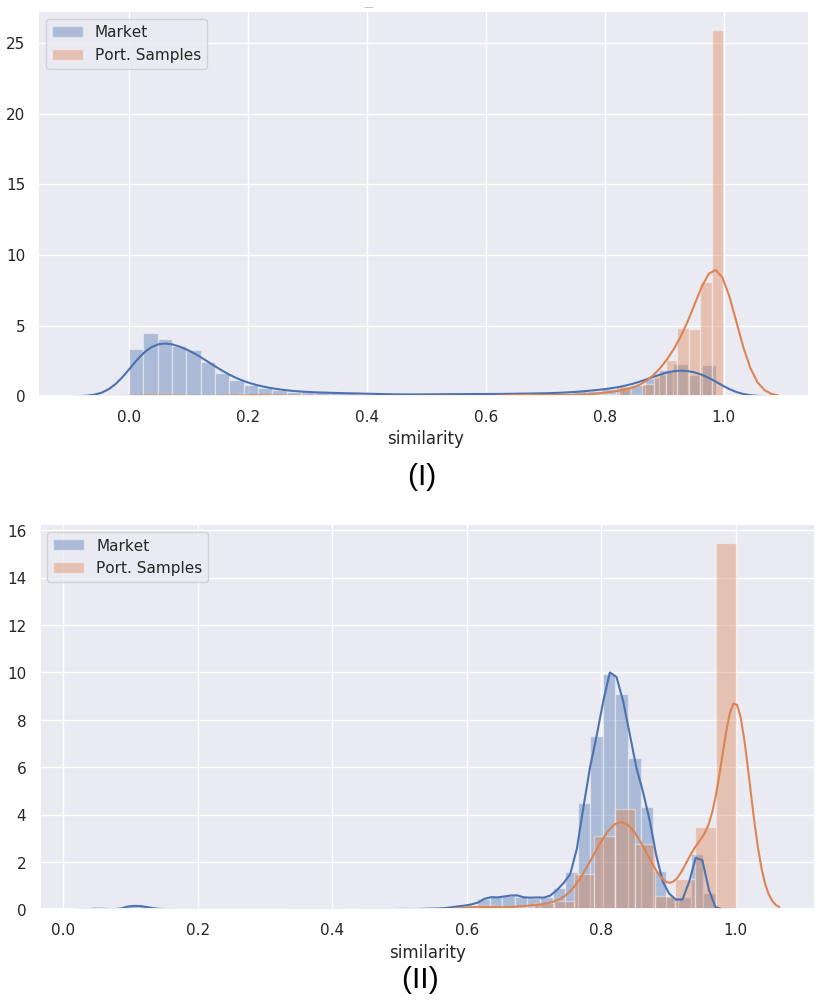
\includegraphics[width=10cm]{fig/ch1-simi-dist-expected-real.png} 
   \caption{Similarity distribution from the benchmark.(I) shows a best case scenario one and (II) a strange-behavior scenario. Source: Author.}
   \label{fig:simi-dist-expected-real}
\end{figure}

This work is one of the several improvements in the On Target product road map. It is a proof of concept which its objective is to analyze whether the overall performance of the high quality leads generation improves by clustering the portfolio before running the recommendation algorithm. 

In order to preserve interpretability, the clustering procedure will not include all available features . Only firmographics variables will be used\cite{wikipedia_firmographics} variables which are related to characteristics of a business, such as: company size, location, number of employees and others.


\section{Objectives}

\subsection{General Objectives}

The general objective of this work is to analyze whether if the performance of the OnTarget improves by clustering the portfolio with firmographics variables before running the recommendation algorithm.

\subsection{Specific Objectives}

Specific objectives of this work are:

\begin{itemize}
    \item defining the clustering strategy;
	\item defining the clustering algorithm;
    \item defining the number of clusters on the studies;
    \item running OnTarget against the benchmark with the clustering approach; and
    \item analyzing similarity distributions and performance metrics against the benchmark.
\end{itemize}


\section{Work outline}

This thesis is organized in the following manner: 

In the chapter 2 some theoretical concepts are explained, so the reader can understand the what theory is behind this work. 

Next, in the chapter 3, is introduced the terms used by the OT's team and a basic view of how it works, later in the chapter, a discussion about the clustering procedures and the conceived experiments.

In chapter 4, is presented the results of these experiments alongside a extensive analysis in the metrics of several scenarios. 
 
Finally, on chapter 5, a recap of this work is presented to the reader, with the takeouts and future work. 